\documentclass[12pt]{article}
\usepackage{graphicx}
\usepackage{caption}

\begin{document}
\begin{titlepage}
\begin{center}
	\textsc{\LARGE Rutgers University}\\[1.5 cm]
    \textsc{\Large Physics 2 lab}\\[0.5cm]
    \rule{\linewidth}{0.5mm} \\ [.4 cm]
    {\huge \bfseries Resistance}\\[.4 cm]
    \rule{\linewidth}{0.5mm} \\ [1.5 cm]
    \begin{minipage}{0.4\textwidth}
	\begin{flushleft} \large
	\emph{Authors:}\\
	Brittney,Kishan,Abhi
	\end{flushleft}
	\end{minipage}
	\begin{minipage}{0.4\textwidth}
	\begin{flushright} \large
	\emph{Teacher:} \\
	James
	\end{flushright}
	\end{minipage}\\[2 cm]
	\textsc{ \Large Signatures} \\[1.7 cm] 
	\rule{10 cm}{0.5mm} \\ [2.0 cm]
	\rule{10 cm}{0.5mm} \\ [2.0 cm]
	\rule{10 cm}{0.5mm}
	\vfill
	{\large {July 27, 2013}}
\end{center}
\end{titlepage}

\section*{Part 1a - resistance of a light-bulb}
\subsection*{Procedure and Goal}
 We have a light-bulb. We send varying amounts of current through the light-bulb. We then measure the voltage across the light-bulb for each current. Our goal is to see if the the resistance of the light-bulb is dependent on the current supplied to it. 

 \begin{figure}[h]
	 \centering
	 \includegraphics[scale = .35]{figOne}
	 \caption{the circuit of our experiment}
  \end{figure}

\subsection*{Prediction}
We can follows these steps to show more current $\Rightarrow$ more resistance

\begin{enumerate}
\item 
More current $\Rightarrow$ brighter light-bulb
\item 
brighter light-bulb $\Rightarrow$ more heat
\item 
more heat  $\Rightarrow$ more resistance
\item 
therefore we can conclude more current $\Rightarrow$ more resistance  
\end{enumerate}
we can say more current $\Rightarrow$ more resistance but can not guess the exact relationship between the current supplied and resistance


\subsection*{Results and Analysis}
Here are the results we achieved.  
\begin{quote}
	\begin{tabular}{|r|r|r|}
	\hline 
	current supplied & voltage across light-bulb & resistance of light-bulb \\
	\hline 
	.03 & .39 & 13 \\
	.04 & .67 & 16.75 \\
	.05 & .98 & 19.6 \\
	.06 & 1.5 & 25 \\
	.07 & 1.93 & 27.5 \\
	.08 & 2.5 & 31 \\
	\hline 
	\end{tabular}
\end{quote}
\begin{figure}[h]
	 \centering
	 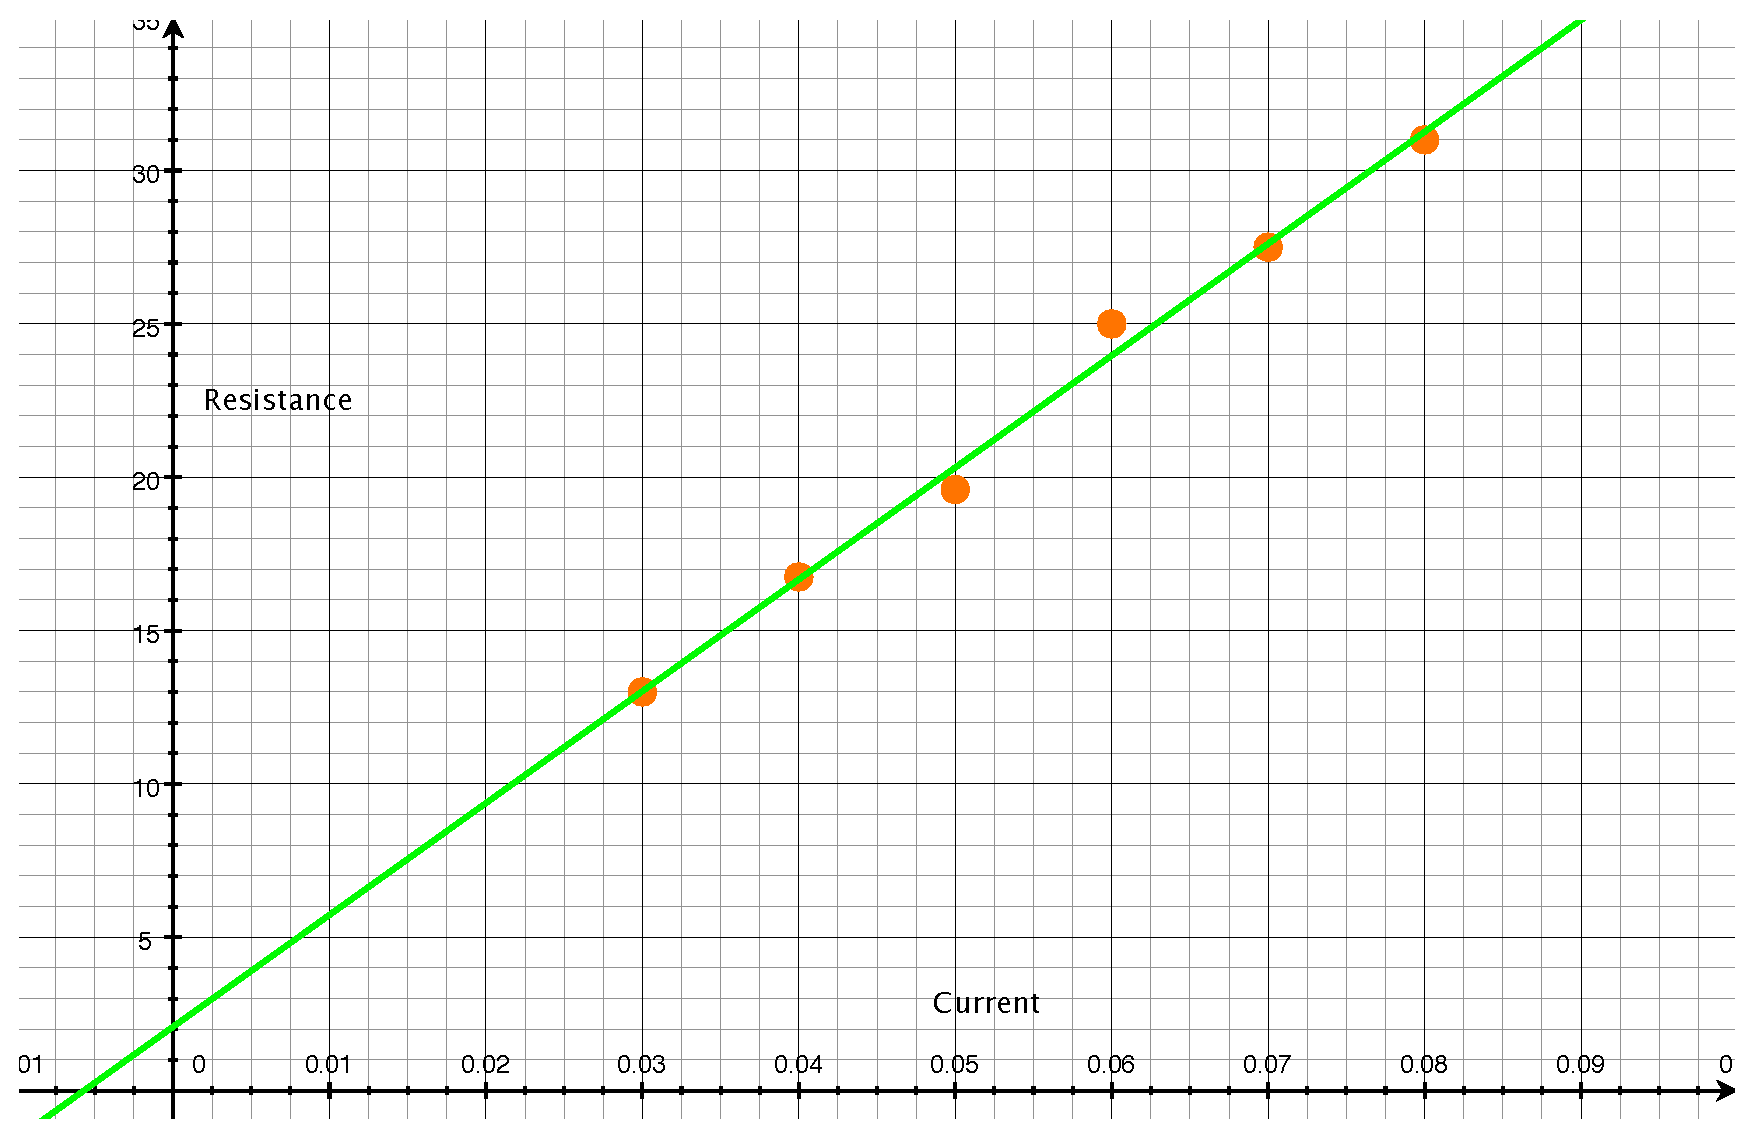
\includegraphics[scale = .51]{graph1}
	 \caption{plotting the resistance as a function of current}
\end{figure}

Our prediction was correct.We found out that the resistance of the light-bulb is directly proportional to the current supplied. The best fit curve we got was $R = 364.71I + 2.08$.
\section*{Part 1b - ohmic resistance}
\subsection*{Procedure and goal}
In this part we repeat part 1a except we replace the light-bulb with a resistance box. We set the box's resistance to 50.
\subsection*{Prediction}
Since by the box has a fixed relationship, there should be no relation between current and resistance. Resistance should stay fixed at 50.
\subsection*{Results and Analysis}
\begin{quote}
	\begin{tabular}{|r|r|r|}
	\hline 
	current supplied & voltage across light-bulb & resistance of light-bulb \\
	\hline 
	.02 & 1 & 50 \\
	.03 & 1.7 & 56.6 \\
	.05 & 2.5 & 50 \\
	.06 & 2.9 & 56.6 \\
	.07 & 3.4 & 55.71 \\
	.08 & 4.3 & 53 \\
	\hline 
	\end{tabular}
\end{quote}
In the second part of this experiment our prediction was correct.  The resistance recorded stayed at around 50, so the box is an ohmic resistor. The
\end{document}